\begin{frame}{Scientific context}
    \textbf{Context :} Create real-time digital twins of an organ (such as the liver).

    \textbf{$\phi$-FEM Method :} New fictitious domain finite element method.

    \begin{enumerate}[\ding{217}]
        \item domain given by a level-set function $\Rightarrow$ don't require a mesh fitting the boundary 
        \item allow to work on complex geometries 
        \item ensure geometric quality 
        % \item Cartesian grid adapted for neural networks
    \end{enumerate}
    
    \begin{center}
        \pgfimage[width=0.65\linewidth]{images/intro/context_geometry.png}
    \end{center}	

    \textit{Practical case:} Real-time simulation, shape optimization...
\end{frame}

\begin{frame}{Objective}
    \textbf{Current Objective :} Develop hybrid finite element / neural network methods.

	\begin{center}
		\begin{tcolorbox}[
			colback=white, % Couleur de fond de la boîte
			colframe=other, % Couleur du cadre de la boîte
			arc=2mm, % Rayon de l'arrondi des coins
			boxrule=0.5pt, % Épaisseur du cadre de la boîte
			breakable, enhanced jigsaw,
			width=0.8\linewidth
			]
			
			\textbf{OFFLINE :}
			
			\begin{figure}[htb]
				\centering
				\resizebox{\textwidth}{!}{%
					\begin{tikzpicture}
						\node at (0,0.8) {Several Geometries};
						\node[draw=none, inner sep=0pt] at (0,0) {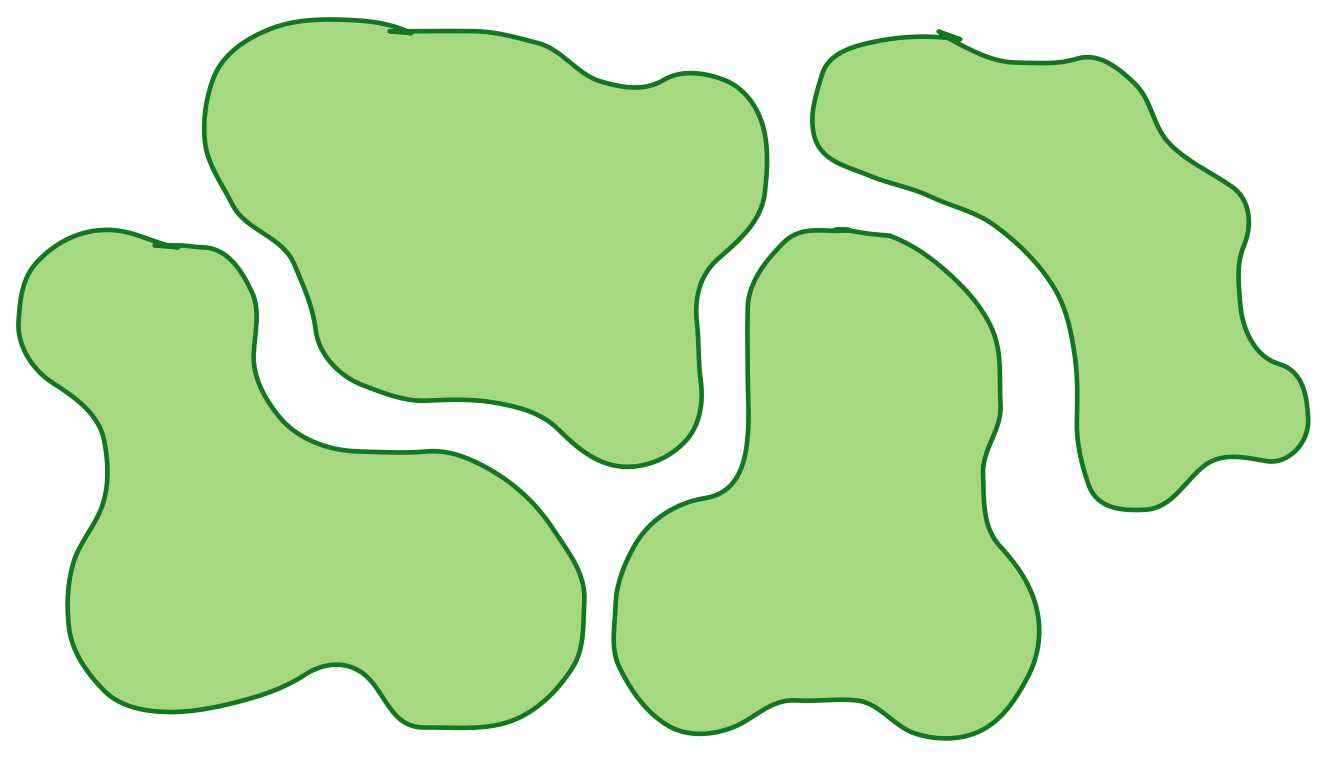
\includegraphics[width=2cm]{images/intro/objective_geom.png}};
						\node[title,font=\Large] at (1.6,0.1) {+};
						\node at (3.5,0.8) {Several Functions};
						\node[draw=none, inner sep=0pt] at (3.5,0) {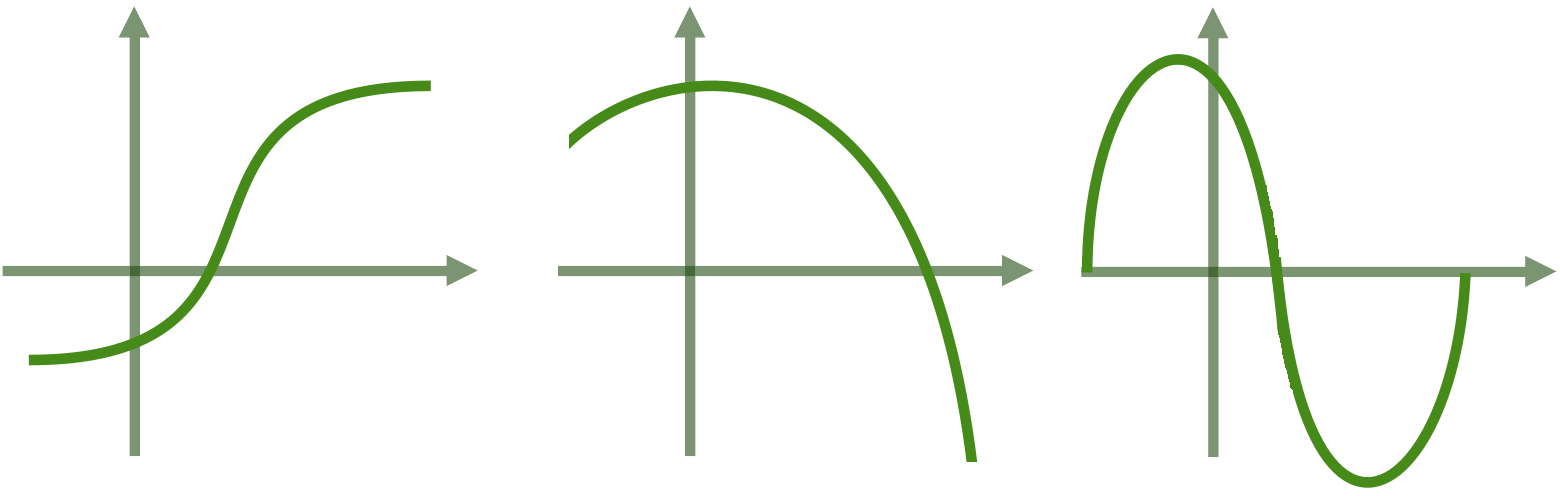
\includegraphics[width=3cm]{images/intro/objective_fct.png}};
						
						% Ajouter une flèche entre les deux rectangles
						\draw[->, title, line width=1.5pt] (5.5,0.1) -- (6.5,0.1);
						%		
						\node at (8,0.8) {Train a PINNs};
						\node[draw=none, inner sep=0pt] at (8,-0.1) {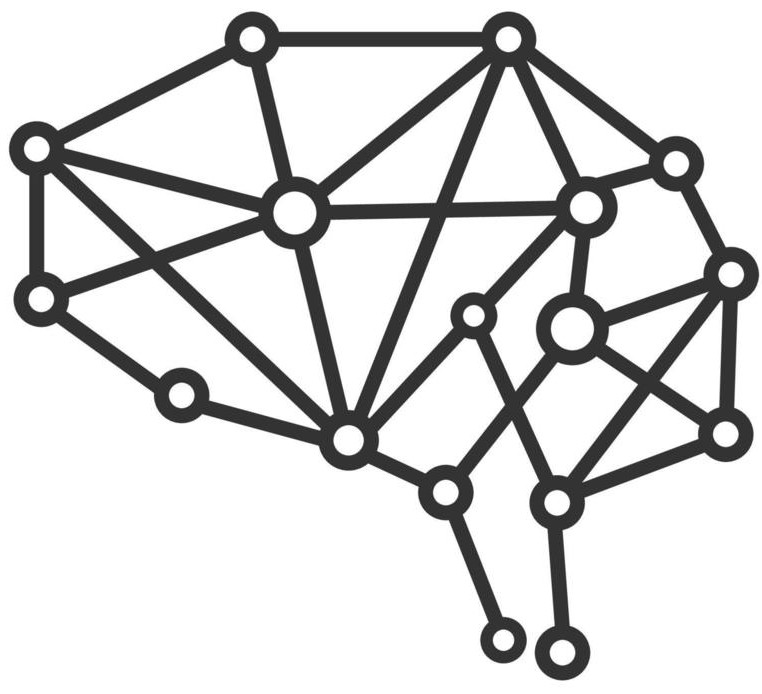
\includegraphics[width=1.5cm]{images/intro/objective_pinns.jpg}};				
					\end{tikzpicture}
				}%
			\end{figure}
			
			\textbf{ONLINE :}
			
			\vspace{-25pt}
			
			\begin{figure}[htb]
				\centering
				\resizebox{\textwidth}{!}{%
					\begin{tikzpicture}
						\node at (0,0.8) {1 Geometry - 1 Function};
						\node[draw=none, inner sep=0pt] at (0,0) {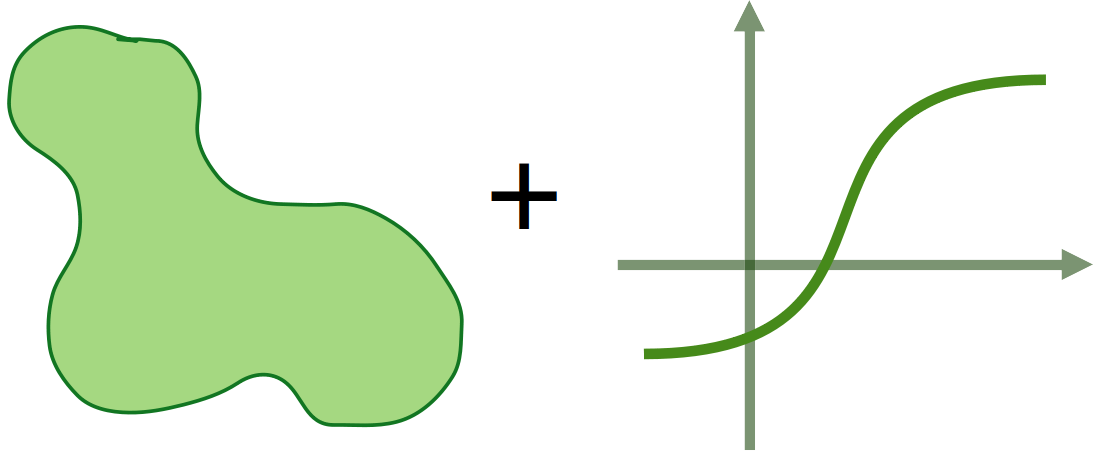
\includegraphics[width=2cm]{images/intro/objective_onegeom_onefct.png}};
						%		\node[title,font=\Large] at (1.6,0.1) {+};
						%		\node at (3.5,0.8) {Several Functions};
						%		\node[draw=none, inner sep=0pt] at (3.5,0) {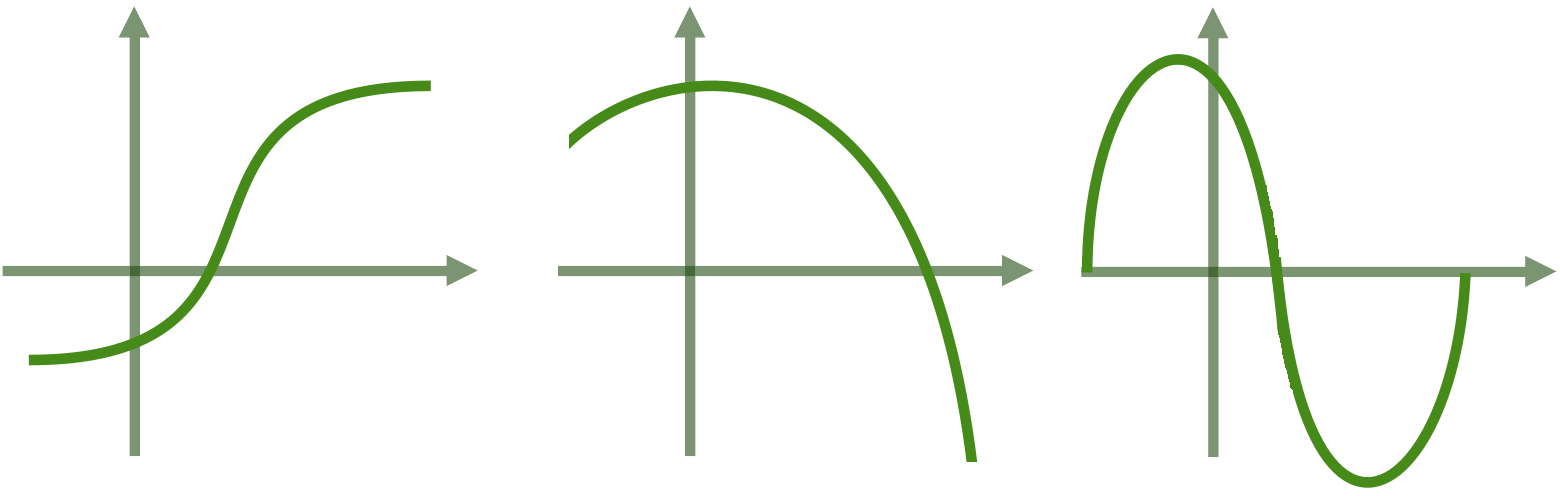
\includegraphics[width=3cm]{images/intro/objective_fct.png}};
						
						\draw[->, title, line width=1.5pt] (2,0.1) -- (3,0.1);
						
						\node[align=center] at (4,1) {Get PINNs \\ prediction};
						\node[draw=none, inner sep=0pt] at (4,-0.1) {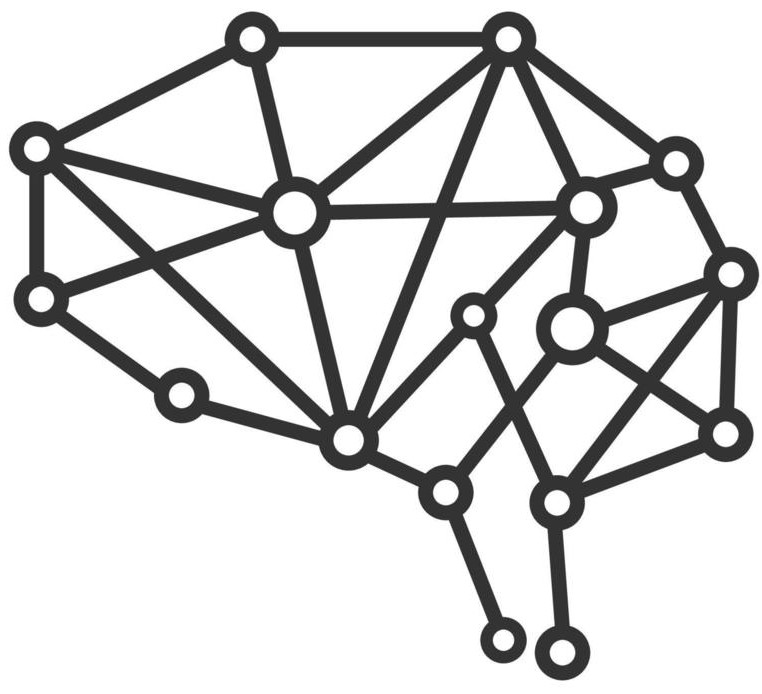
\includegraphics[width=1.5cm]{images/intro/objective_pinns.jpg}};
						
						% Ajouter une flèche entre les deux rectangles
						\draw[->, title, line width=1.5pt] (5.5,0.1) -- (6.5,0.1);
						%		
						\node[align=center] at (8,1) {Correct prediction \\ with $\phi$-FEM};
						\node[draw=none, inner sep=0pt] at (8,-0.1) {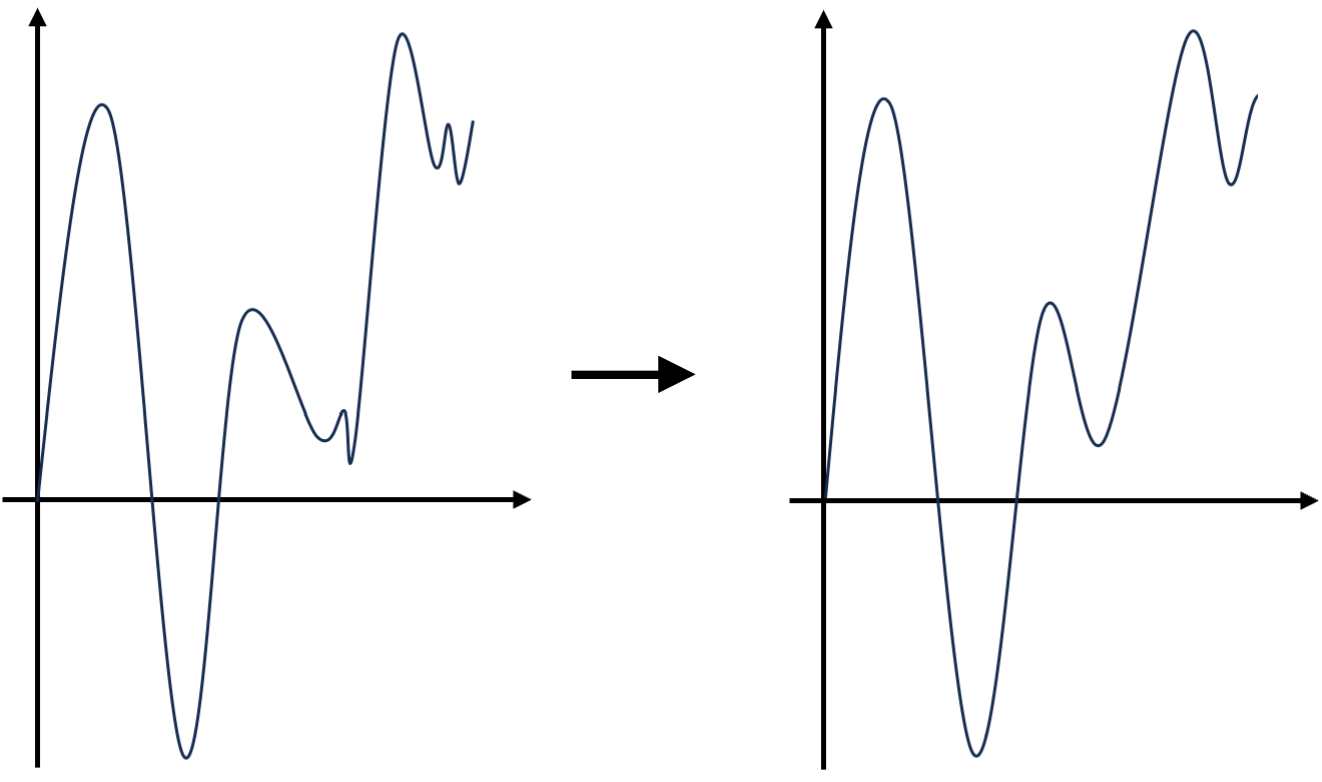
\includegraphics[width=2.5cm]{images/intro/objective_corr.png}};		
					\end{tikzpicture}
				}%
			\end{figure}
		\end{tcolorbox}
	\end{center}

    \textbf{Evolution :}

    \small
    % \setstretch{0.5}
    \begin{itemize}
        \item Geometry : 2D, simple, fixed (as circle, ellipse..) $ \; \rightarrow \;$ 3D / complex / variable
        \item PDE : simple, static (Poisson problem) $\; \rightarrow \;$ complex / dynamic (elasticity, hyper-elasticity)
        \item Neural Network : simple and defined everywhere (PINNs) $\; \rightarrow \;$ Neural Operator
    \end{itemize}
\end{frame}

\begin{frame}{Problem considered}
    \textbf{Elliptic problem with Dirichlet conditions :} \\
    Find $u : \Omega \rightarrow \mathbb{R}^d (d=1,2,3)$ such that
    \begin{equation}
    	\left\{\begin{aligned}
    		&L(u)=-\nabla \cdot (A(x) \nabla u(x)) + c(x)u(x) = f(x) \quad \text{in } \Omega, \\
    		&u(x) = g(x) \quad \text{on } \partial \Omega
    	\end{aligned}\right. \label{edp}
    \end{equation}
	with $A$ a definite positive coercivity condition and $c$ a scalar. We consider $\Delta$ the Laplace operator, $\Omega$ a smooth bounded open set and $\Gamma$ its boundary. 
    
    \textbf{Weak formulation :}
    \begin{equation*}
    	\text{Find } u\in V \text{ such that } a(u, v) = l (v) \forall v\in V
    \end{equation*}
    
    with
    \begin{align*}
    	a(u,v)&=\int_{\Omega} (A(x)\nabla u(x)) \cdot \nabla v(x) + c(x)u(x)v(x) \, dx \\
    	l(v)&=\int_{\Omega} f(x)v(x) \, dx
    \end{align*}
    
    \footnotesize
    \textit{Remark :} For simplicity, we will not consider 1st order terms. 

%    We will define by
%    \begin{equation*}
%        ||u_{ex}-u_{method}||_{0,\Omega}^{(rel)}=\frac{\int_\Omega (u_{ex}-u_{method})^2}{\int_\Omega u_{ex}^2}
%    \end{equation*}
%    the relative error between
%    \begin{itemize}
%        \item $u_{ex}$ : the exact solution  
%        \item $u_{method}$ : the solution obtained by a method \\
%        (can be : FEM or $\phi$-FEM, a correction solver or the prediction of an neural network).
%    \end{itemize}
\end{frame}

\begin{frame}{Numerical methods}
	\textbf{Objective :} Show that the philosophy behind most ofd the methods are the same.
	\begin{center}
		Mesh-based methods \hspace{5pt} // \hspace{5pt} Physically informed learning
	\end{center}
	
	\textbf{Numerical methods :} Discrete an infinite-dimensional problem (unknown = function) and solve it in a finite-dimensional space (unknown = vector).
	\begin{enumerate}[\textbullet]
		\item \textbf{Encoding :} we encode the problem in a finite-dimensional space
		\item \textbf{Approximation :} solve the problem in finite-dimensional space
		\item \textbf{Decoding :} bring the solution back into infinite dimensional space
	\end{enumerate}
	
	\begin{center}
		\begin{tabular}{|c|c|c|}
			\hline
			\textbf{Encoding} & \textbf{Approximation} & \textbf{Decoding} \\
			\hline
			$f \; \rightarrow \theta_f$ & $\theta_f \; \rightarrow \theta_u$ & $\theta_u \; \rightarrow u_\theta$ \\
			\hline
		\end{tabular}
	\end{center}
\end{frame}
